%% LyX 2.0.6 created this file.  For more info, see http://www.lyx.org/.
%% Do not edit unless you really know what you are doing.
\documentclass[english]{article}
\usepackage[T1]{fontenc}
\usepackage[latin9]{inputenc}
\usepackage{graphicx}
\usepackage{babel}
\begin{document}

\title{Exercise 5-3}


\author{Richel Bilderbeek}

\maketitle

\subsubsection*{a) Clutch size}

Clutch size for no abortion:

\[
C(a=0)=\frac{E}{\frac{1}{2}e_{s}+\frac{1}{2}e_{d}}
\]


Clutch size for full abortion:

\[
C(a=1)=\frac{E}{\frac{1}{2}e_{a}+\frac{1}{2}e_{d}}
\]


Clutch size in general:

\[
C(a)=\frac{E}{\frac{1}{2}(a.e_{a}+(1-a)e_{s})+\frac{1}{2}e_{d}}
\]


\[
C(a)=\frac{2E}{a.e_{a}+(1-a)e_{s}+e_{d}}
\]



\subsubsection*{b) Secondary sex ratio}

Secondary sex ratio for no abortion:

\[
S(a=0)=\frac{sons}{sons+daughters}=\frac{\frac{1}{2}}{\frac{1}{2}+\frac{1}{2}}=\frac{1}{2}
\]


Secondary sex ratio for full abortion:

\[
S(a=1)=\frac{sons}{sons+daughters}=\frac{0}{0+\frac{1}{2}}=0
\]


Secondary sex ratio in general:

\begin{equation}
S(a)=\frac{sons}{sons+daughters}=\frac{\frac{1}{2}-\frac{1}{2}a}{\frac{1}{2}-\frac{1}{2}a+\frac{1}{2}}=\frac{1-a}{2-a}\label{eq:S}
\end{equation}



\subsubsection*{c) Calculate a mutant its fitness}

Shaw-Mohler equation, with $x$ replaced by $a$:

\begin{equation}
W(a,a^{*})=\frac{1}{2}\left[\frac{m(a)}{m(a^{*})}+\frac{f(a)}{f(a^{*})}\right]\label{eq:ShawMohler}
\end{equation}


To solve this, we need $m(a)$ and $f(a)$:

\[
m(a)=C(a)s(x)P_{s}(a)=C(a)\frac{1}{2}(1-a)=C(a)\left[\frac{1}{2}-\frac{1}{2}a\right]
\]


\[
f(a)=C(a)s(x)P_{d}(a)=C(a)\frac{1}{2}.1=\frac{1}{2}C(a)
\]


Filling this in:

\begin{equation}
W(a,a^{*})=\frac{1}{2}\left[\frac{C(a)[\frac{1}{2}-\frac{1}{2}a]}{C(a^{*})[\frac{1}{2}-\frac{1}{2}a^{*}]}+\frac{\frac{1}{2}C(a)}{\frac{1}{2}C(a^{*})}\right]=\frac{1}{2}.\frac{C(a)}{C(a^{*})}\left[\frac{1-a}{1-a^{*}}+1\right]\label{eq:FitnessMutant}
\end{equation}



\subsubsection*{d) For $e_{a}<e_{d}$, Is the equal allocation principle still valid?}

This equation should work, for the equal allocation principle to be
valid:

\[
\frac{s^{*}}{1-s^{*}}=\frac{e_{d}}{e_{s}}
\]


Too bad, this does not take into account the cost of abortion. So,
using equation \ref{eq:S} to determine the abortion strategy:

\[
\frac{s^{*}}{1-s^{*}}=\frac{\frac{1-a^{*}}{2-a^{*}}}{1-\frac{1-a^{*}}{2-a^{*}}}=1-a^{*}
\]


In section (g) we calculate $a^{*}$, so we can plug it in:

\begin{equation}
\frac{s^{*}}{1-s^{*}}=1-a^{*}=1-\left[\frac{-e_{s}+e_{d}+2.e_{a}}{e_{a}-e_{s}}\right]=\frac{e_{d}+e_{a}}{e_{s}-e_{a}}\label{eq:EAP_with_abortion}
\end{equation}


Now we can see that abortion is an investment at the expense of sons
(see the denominator) at the gain of daughters (numerator). Taking
into account abortion, the equal allocation principle is still unscathed. 


\subsubsection*{e) For $e_{a}=e_{d}$, is the equal allocation principle still valid?}

From equation \ref{eq:EAP_with_abortion} we can see that abortion
is invested in the creation of daughters. If this investment (the
expense of a son) equals its return (a daughter), nothing is gained
by aborting sons.


\subsubsection*{f) Plot of a graph}

Using equation \ref{eq:a_star} (which is derived below).

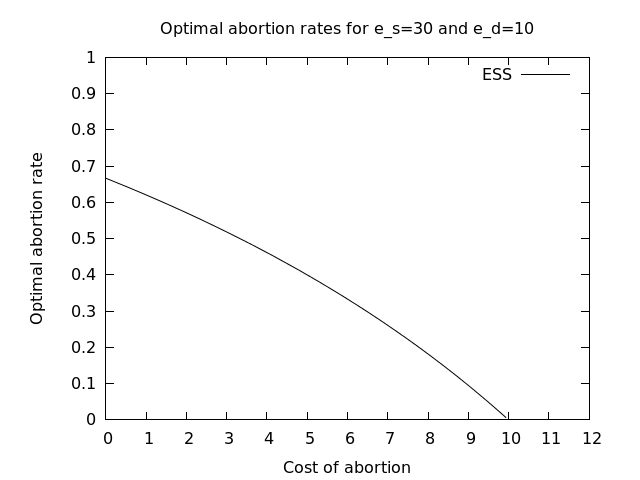
\includegraphics[scale=0.5]{Day5_3_plot}


\subsubsection*{g) Derive $a^{*}$}

First equation \ref{eq:FitnessMutant} needs to be reworked before
taking the partial differential of $W(a,a^{*})$ to $a$:

\[
W(a,a^{*})=\frac{1}{2}.\frac{C(a)}{C(a^{*})}\left[\frac{1-a}{1-a^{*}}+1\right]=\left[\frac{E}{1-a^{*}C(a^{*})}\right]\left[\frac{2-a-a^{*}}{a.e_{a}+(1-a)e_{s}+e_{d}}\right]
\]


Because the first term is indepent of $a$, it does not take part
in the partial differential:

\[
k=\left[\frac{E}{1-a^{*}C(a^{*})}\right]
\]


Extracting $k$ and differentiating with the quotient rule:

\[
\left[\frac{f}{g}\right]^{'}=\frac{f'g-f.g'}{(g)^{2}}=\frac{dW}{da}=\frac{e_{s}-e_{d}-2.e_{a}+a^{*}.e_{a}-a^{*}.e_{s}}{(g)^{2}}
\]


To find the maximum $k\frac{dW}{da}=0$ must be solved, of which either
$k$ or $\frac{dW}{da}$is zero:

\[
k=\left[\frac{E}{1-a^{*}C(a^{*})}\right]=0
\]


\begin{equation}
a^{*}=\frac{-e_{s}-e_{d}}{e_{a}-e_{s}}\label{eq:a_star_nonsense}
\end{equation}


\[
\frac{dW}{da}=0
\]


\[
e_{s}-e_{d}-2.e_{a}+a^{*}.e_{a}-a^{*}.e_{s}=0
\]


\begin{equation}
a^{*}=\frac{-e_{s}+e_{d}+2.e_{a}}{e_{a}-e_{s}}\label{eq:a_star}
\end{equation}


Note that equation \ref{eq:a_star_nonsense} is mathematically valid,
but only works when some costs are negative.


\subsubsection*{Acknowledgements}

The author would like to thank Anna Depetris and Francesca Sozzi for
their collaboration.
\end{document}
